\documentclass[border=5pt]{standalone}
\usepackage{tikz}
\usepackage{amsmath}
\begin{document}
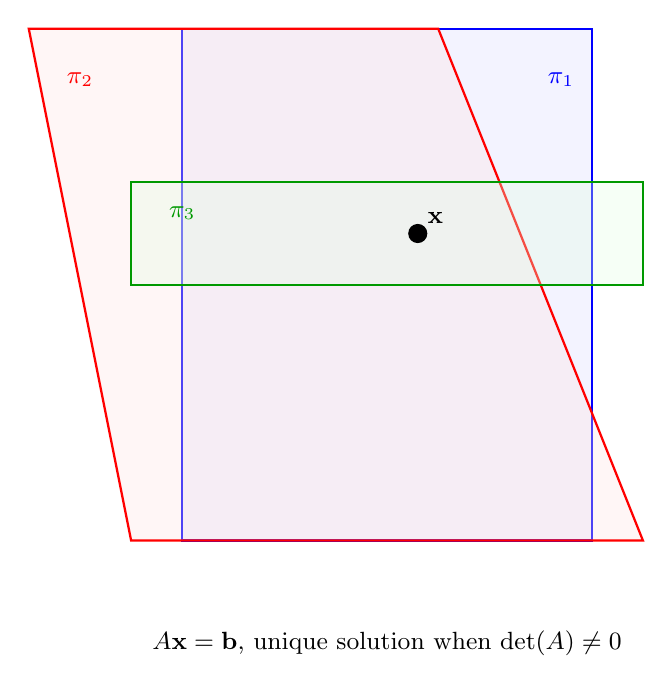
\begin{tikzpicture}[scale=1.3, >=stealth]
  % Unique solution: intersection of 3 planes

  % Plane 1 (blue, vertical-ish)
  \fill[blue!12, opacity=0.4] (-1.5,-2) -- (2.5,-2) -- (2.5,3) -- (-1.5,3) -- cycle;
  \draw[thick, blue] (-1.5,-2) -- (2.5,-2) -- (2.5,3) -- (-1.5,3) -- cycle;
  \node[blue, font=\small] at (2.2, 2.5) {$\pi_1$};

  % Plane 2 (red, tilted)
  \fill[red!12, opacity=0.3] (-2,-2) -- (3,-2) -- (1,3) -- (-3,3) -- cycle;
  \draw[thick, red] (-2,-2) -- (3,-2) -- (1,3) -- (-3,3) -- cycle;
  \node[red, font=\small] at (-2.5, 2.5) {$\pi_2$};

  % Plane 3 (green, horizontal-ish)
  \fill[green!12, opacity=0.3] (-2,0.5) -- (3,0.5) -- (3,1.5) -- (-2,1.5) -- cycle;
  \draw[thick, green!60!black] (-2,0.5) -- (3,0.5) -- (3,1.5) -- (-2,1.5) -- cycle;
  \node[green!60!black, font=\small] at (-1.5, 1.2) {$\pi_3$};

  % Intersection point
  \filldraw[black] (0.8, 1) circle (2.5pt);
  \node[font=\small, above right] at (0.8, 1) {$\mathbf{x}$};

  % Formula
  \node[font=\small] at (0.5, -3) {$A\mathbf{x} = \mathbf{b}$, unique solution when $\det(A) \neq 0$};
\end{tikzpicture}
\end{document}
